The objectives of our empirical study are the following:
\begin{itemize}
\item \textbf{OBJ1:} To evaluate the encumbrance (execution time, memory, storage) of \textbf{L-ISR} on both GPU and CPU on a modern supercomputer.
\item \textbf{OBJ2:} To evaluate the efficacy of \textbf{L-ISR-PHE} for the \textbf{EUS} problem.
\end{itemize}
%
%Our empirical study evaluates and presents: 1) in situ encumbrance for varying particle workloads, and 2) a detailed quantitative evaluation of the Lagrangian representation.
%%
%Thus, we conduct experiments to measure both.
%%
%Each experiment reports the costs of in situ extraction of a Lagrangian representation. 
%%
%For tests that are measuring reconstruction quality, a post hoc reconstruction phase is involved.
%%
%We do not perform post hoc reconstruction in a limited set of cases due to a limited compute node-hour allocation.

In the following subsections, we describe all the components of our empirical study.
%
We discuss the infrastructure and implementations we use~(\ref{sec:infra}), the runtime environment specifics~(\ref{sec:runtime}), the parameter space we explore~(\ref{sec:parameters}), the simulation codes~(\ref{sec:datasets}), and finally, our evaluation of in situ encumbrance~(sec:encumbrance) and reconstruction accuracy~(\ref{sec:evaluation}).
%
Table~\ref{table:notation} provides a list of notations we use in this empirical study (Step, DAV\%, Interval, 1:X, L-ISR-PHE, EUS, Avg$_{L2}$, Max$_{L2}$).


\subsection{Infrastructure and Implementation}
\label{sec:infra}
\subsubsection{In Situ}
\label{sec:insituimp}
We use the Ascent~\cite{larsen2017alpine} \textit{in situ} infrastructure and VTK-m~\cite{moreland2016vtk} library to implement \textit{in situ} data reduction via by calculating a Lagrangian representation. 
%
%Lagrangian analysis is implemented as an extraction filter in VTK-m. 
%
%For each of the simulation codes we consider, Ascent is first integrated with the simulation code.
%
%Ascent can be configured to perform Lagrangian analysis when the simulation is executed.
%
%The specifics of an analysis configuration are input to Ascent using either a json or yaml file.
%
%The Lagrangian analysis filter requires parameters specifying seed resolution, frequency of storing information to disk, the name of the vector field, and step size.
%%
%Ascent passes the simulation velocity data to the Lagrangian filter via VTK-h~\cite{larsen2017alpine}, a distributed memory wrapper around VTK-m, every cycle. 
%
%Further, we use utilities within Ascent to measure timings and to strip simulation data of ghost zones.
%
The VTK-m Lagrangian filter on each rank operates independently and maintains its own list of basis particles and uses the existing particle advection infrastructure available in VTK-m~\cite{pugmire2018performance}.
%
RK4 particle advection is implemented using VTK-m worklets (kernels or functors) that offer performance portability by utilizing the underlying hardware accelerators. 
%
%The Lagrangian filter operates across simulation cycles and stores one value in memory for each basis flow seed particle: current position (x, y, z).
%
In our implementation, each Lagrangian filter stores the displacement of each particle (3 double), as well as its validity (1 boolean), i.e., whether the particle remained within the domain during the interval of calculation.
%
%The validity of a particle is essential to consider when searching for a valid interpolation neighborhood during post hoc reconstruction.
%
%Our implementation computes the displacement and validity using VTK-m worklets as a final step before adding both fields to the output data set object. 
%
In more complicated frameworks, it is possible to associate additional information (for example, ID, age, start location, previous locations, etc.) with each particle at the cost of higher runtime memory usage and data storage.
%
%For our study, we store data in a VTK ASCII file format for structured grids.
%
%Figure~\ref{} is a schematic diagram of the infrastructure and shows the relation of \textit{in situ} Lagrangian analysis to the simulation code.

We use Ascent to store the complete velocity field at a specified frequency in order to evaluate the traditional Eulerian paradigm.
%
%Similar to the Lagrangian filter, we store data in a VTK ASCII file format for structured grids.
%
For every Eulerian configuration, we store the full spatial resolution of the simulation domain under consideration. 
%

\subsubsection{Post Hoc}
We build two parallelize-over-data distributed-memory \textit{post hoc} interpolation pipelines, one for each: Lagrangian and Eulerian.
%
%To calculate pathlines using the Lagrangian data post hoc, a particle $p$ identifies a neighborhood of basis flows to follow.
%
%A neighborhood is the convex hull that contains the location of the $p$.
%
For the Lagrangian \textbf{PHE} we construct a search structure in the form of a Delaunay triagulation over the start locations of valid basis particles using CGAL~\cite{fabri2011cgal} to identify particle neighborhoods.
%We calculate the Delaunay triangulation over all the start locations of valid basis flows using CGAL~\cite{fabri2011cgal}.
%
%Thus, we locate particle neighborhoods by identifying the containing cell in the Delaunay triangulation. 
%
%We choose to use a reconstruction method that can operate on structured, as well as unstructured data, because Lagrangian representations can take many forms.
%
%Use of a method that supports unstructured input, i.e., the basis particles are not initialized along a uniform grid, provides a better representation of the general post hoc reconstruction case.
%
%The most straightforward, albeit expensive, approach is to calculate a global Delaunay triangulation.
%
%However, a global Delaunay triangulation can get prohibitively expensive as the total number of particles increases.
%
%A second approach is to perform spatial binning followed by a smaller more local Delaunay triangulation.
%
%However, this method requires an expanding search structure in addition to a binning scheme to guarantee a particle locates a neighborhood if available.
%
%Further, the cost of calculating a local Delaunay triangulation for each particle would be dependent on the number of particles.
%
In our implementation, each rank loads basis particles of the rank itself as well as basis particles generated by spatially adjacent ranks (i.e., upto 27 ranks for a rectilinear simulation grid).
%
%Thus, each post hoc interpolation rank loads data from upto 27 ranks.
%
%The Delaunay triangulation is then performed for all the valid basis flows in the loaded data.
%
%Although not optimal, this approach will scale better than a global Delaunary triangulation while remaining straightforward.
%
%The best approach to identify a particle neighborhood in a large distributed memory settings with a large number of particles remains an open research problem and is beyond the scope of this work. 
%
Once a particle neighborhood is identified, barycentric coordinate interpolation is used to calculate the displacement of $p$.  
%
%If a particle enters the domain bounds of an adjacent node it is communicate to the rank corresponding to that domain using MPI. 
%
Our implementation uses MPI to communicate particles across ranks and continue the integration of trajectories across node boundaries.

For the Eulerian \textit{post hoc} interpolation pipeline, we use the VTK-m particle advection infrastructure to perform RK4 integration and MPI for communication of particles across ranks.
%
%In this pipeline, each rank is only required to load the velocity field stored to disk for that particular rank.


\subsection{Runtime Environment}
\label{sec:runtime}
Our empirical study used two machines: Summit and Alaska. 
%
Summit is a supercomputer at ORNL. 
%
A Summit compute node has two IBM Power9 CPUs, each with 21 cores running at 3.8 GHz and 512 GBytes of DDR4 memory. 
%
Nodes on Summit also have enhanced on-chip acceleration with each CPU connected via NVLink to 3 GPUs, for a total of 6 GPUs per node. 
%
Each GPU is an NVIDIA Tesla V100 with 5120 CUDA cores, 6.1 TeraFLOPS of double precision performance, and 16 GBytes of HBM2 memory.
%
Lastly, it uses a Mellanox EDR 100G InfiniBand, Non-blocking Fat Tree as its interconnect topology.

Alaska is the small cluster at our research lab.
%
The head node with consists of two Intel Xeon E5-2667v3 CPU, each with 16 cores running at 3.2 GHz. 

We use Summit to build, integrate, and execute in situ Lagrangian analysis with simulation codes.
%
Thus, all of our in situ extraction is performed on Summit. 
%
Additionally, we use Summit to perform large distributed memory post hoc reconstructions.
%
We use Alaska for the smaller post hoc reconstruction processes.


\subsection{Parameter Space}
\label{sec:parameters}

We vary the different ``knobs'' in the parameter space to evaluate the viability and efficacy of using in situ Lagrangian analysis to perform exploratory time-dependent vector field analysis and visualization. 
%
We consider the following parameters:
\begin{itemize}
\item \textbf{Number of particles:} Our study varies the number of particles initialized per node and thus inform the cost of performing particle advection for varying workloads every cycle of the simulation. Further, the number of particles initialized is directly impacts the size of the data stored to disk and the accuracy of the reconstruction.
%
We specify the number of particles initialized using the notation \textbf{1:X}, where X is the reduction factor. 
%
For example, a 1:1 configuration states that one particle is used for every grid point (no reduction) and a 1:8 configuration states that one particle is used for every 8 grid points (12.5\% of the original data size). 
%
\item \textbf{Interval:} We consider the interval or frequency at which files are stored to disk. 
%
For a given total number of simulation cycles, this impacts the total amount of data stored to disk. 
%
Additionally, for the Lagrangian representation, the interval is directly related to the integration length of each massless particle. 
%
For each configuration, we specify the number of cycles between storing to disk and refer to this as the \textbf{interval}. 
%
\item \textbf{Simulation code:} We consider three different time-dependent vector fields produced by simulation codes. Further, we vary the size of the simulation code to gauge the variation in cost for in situ Lagrangian analysis. 
\item \textbf{Scale and Parallelization Hardware:} We consider the costs at various scale (i.e., number of compute nodes, MPI ranks). Further, the simulation codes required different parallelization hardware and thus, across simulation codes we demonstrate in situ Lagrangian analysis using, both, GPU and CPU for particle advection.
\end{itemize}

%Most of our experiment test configurations have two phases: in situ and post hoc. 
%
%The performance characteristics of the in situ phase is what we are primarily interested in.
%
%We execute extra ``only-extraction'' configurations to gauge in situ performance and that do not continue to the post hoc phase.
%
%The post hoc phase in our study is used to measure accuracy.
%
%We report timings associated with performing post hoc Lagrangian reconstruction on a single node and in a distributed memory setting.
%
%We strongly believe that as in situ Lagrangian representations evolve, the post hoc techniques used will as well.
%
%Currently, to the best of our knowledge there does not exist a perfect one-size-fits-all post hoc Lagrangian-based advection method.

%\begin{figure}[t]
\centering
%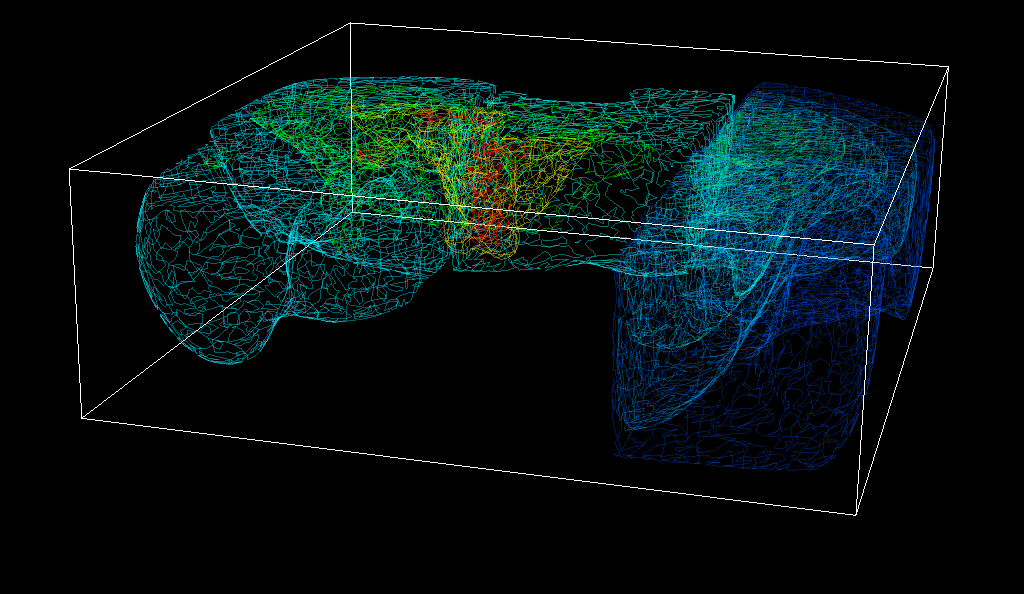
\includegraphics[width=0.8\linewidth]{images/sw4_vis_2.png}
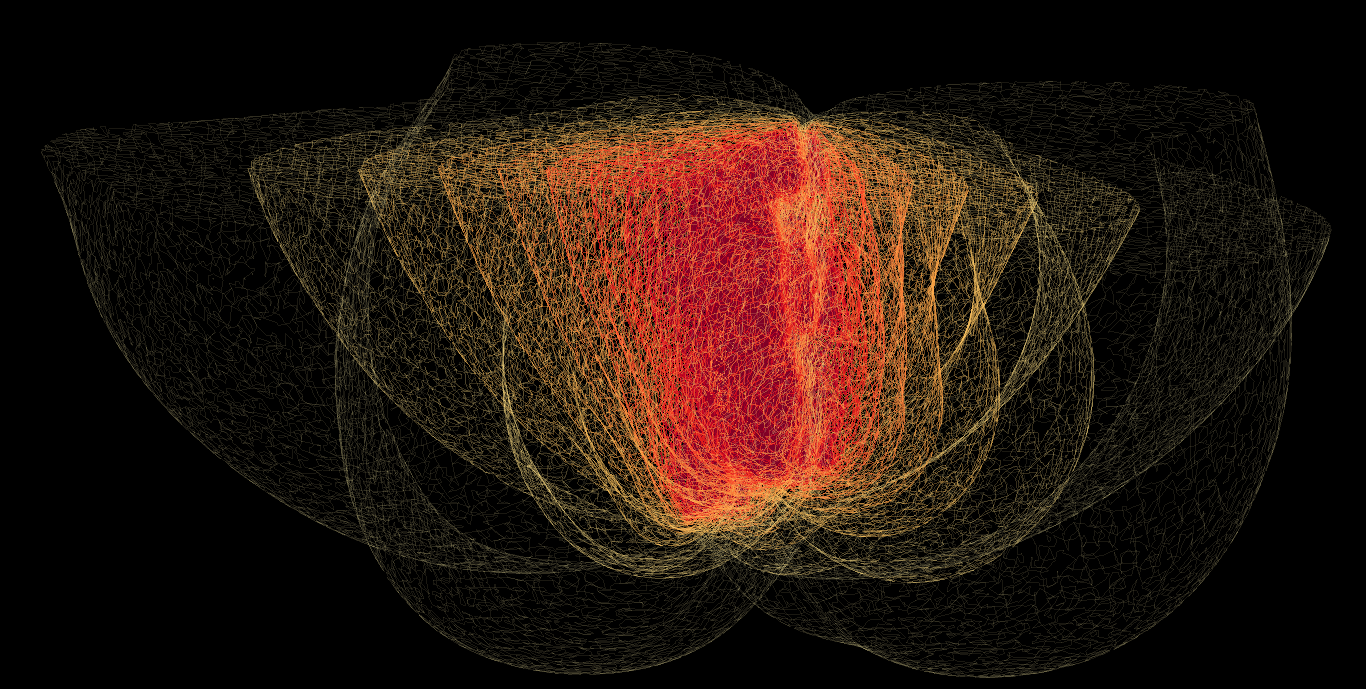
\includegraphics[width=0.8\linewidth]{images/sw4_waves.png}
\caption{SW4 wave propagation visualization}
\label{fig:sw4_vis}
\end{figure}



%\begin{figure}[t]
\centering
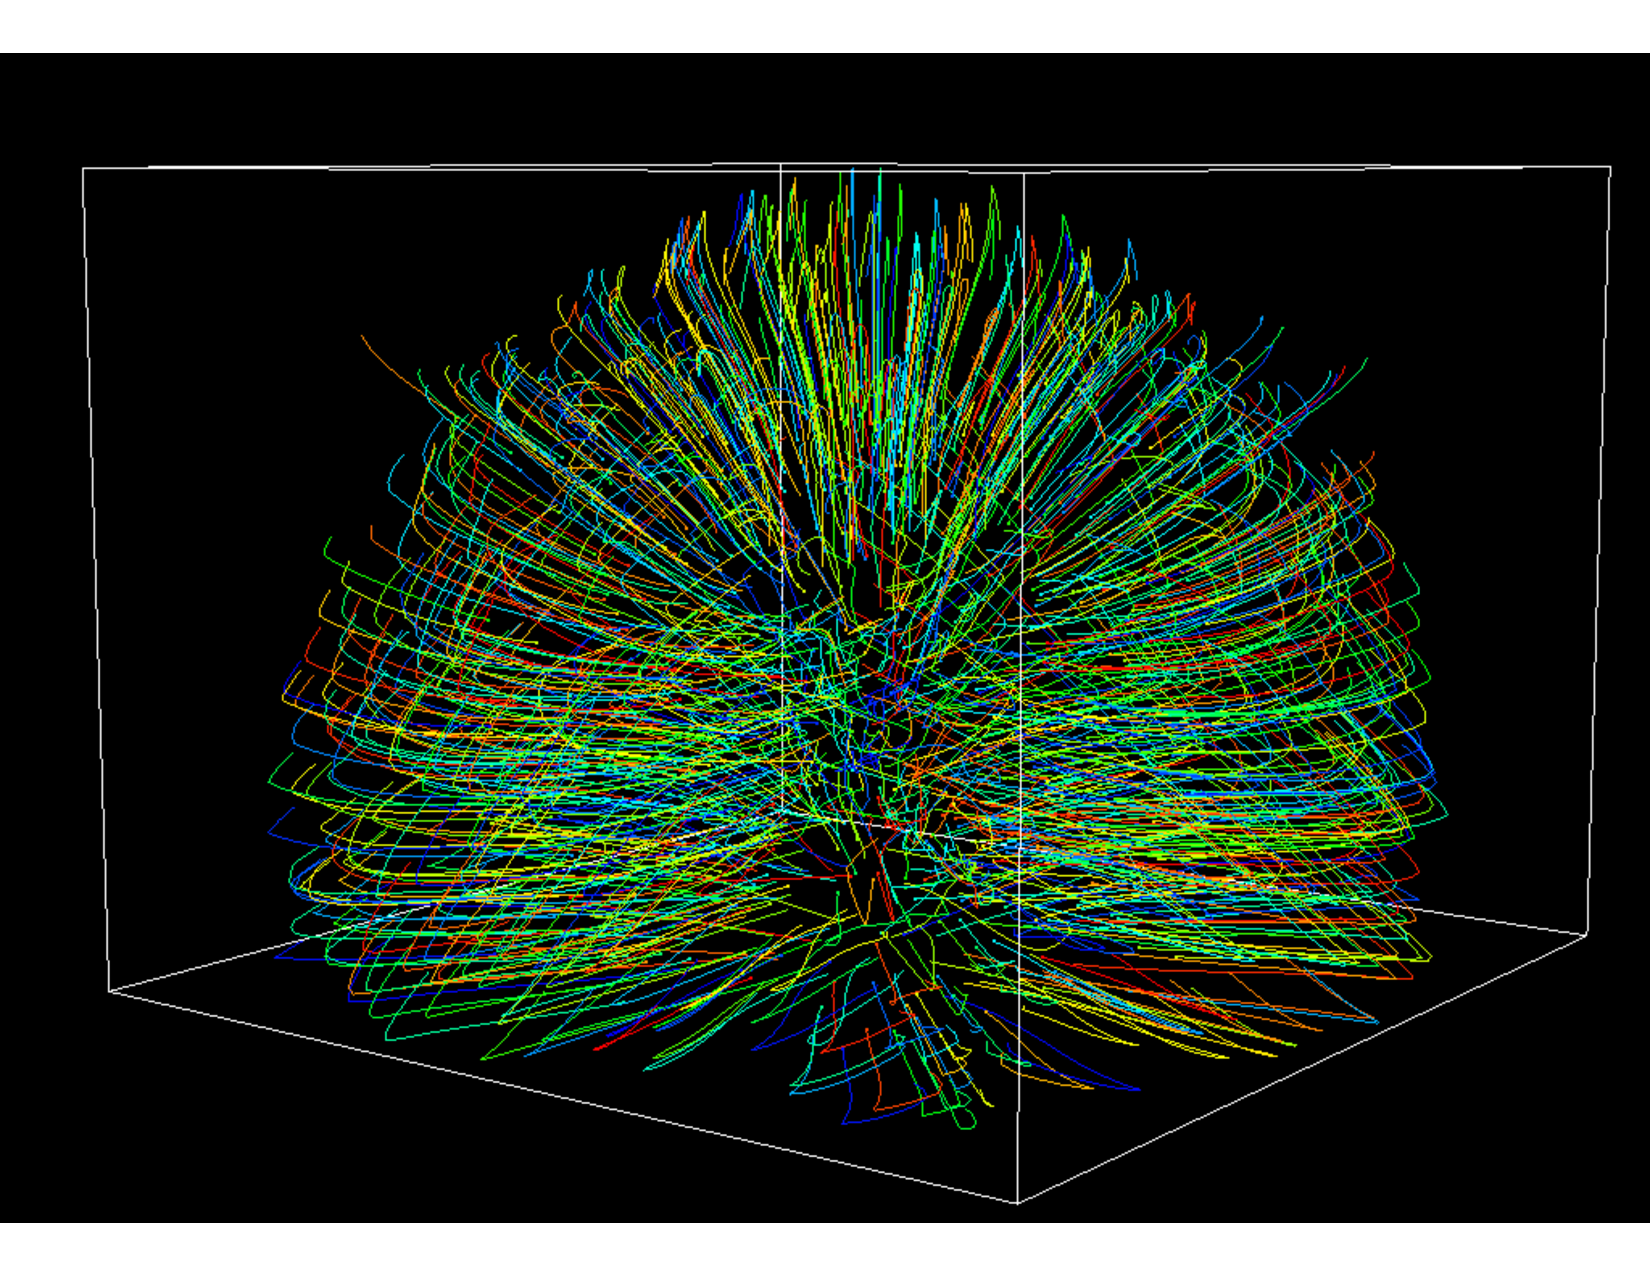
\includegraphics[width=0.7\linewidth]{images/pathlines_clover.pdf}
\caption{Cloverleaf3D flow visualization}
\label{fig:pathlines_clover}
\end{figure}



%\begin{figure}[t]
\centering
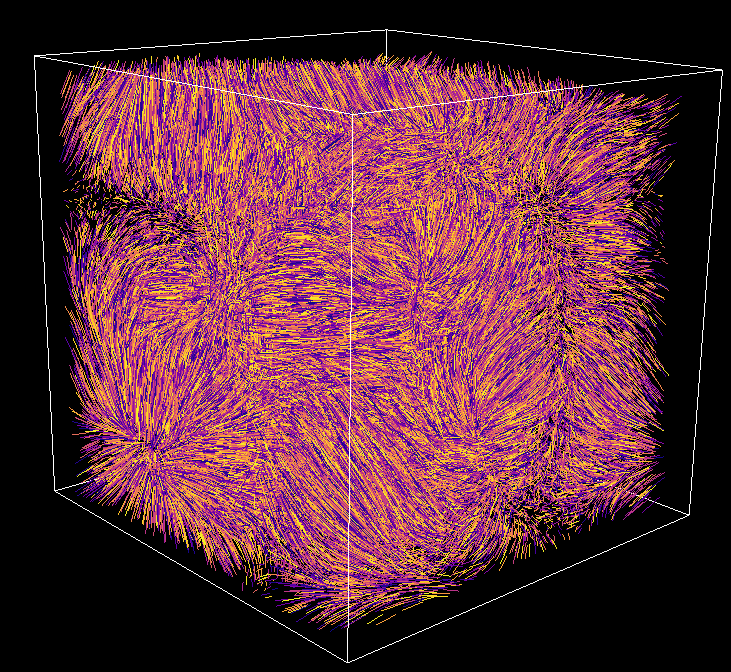
\includegraphics[width=0.65\linewidth]{images/pathlines_nyx.png}
\caption{Nyx flow visualization: 100,000 randomly seeded pathlines calculated for the first 25 cycles of the simulation.}
\label{fig:pathlines_nyx}
\end{figure}



\begin{figure*}[ht]
\centering
\begin{subfigure}{0.27\textwidth}
\centering
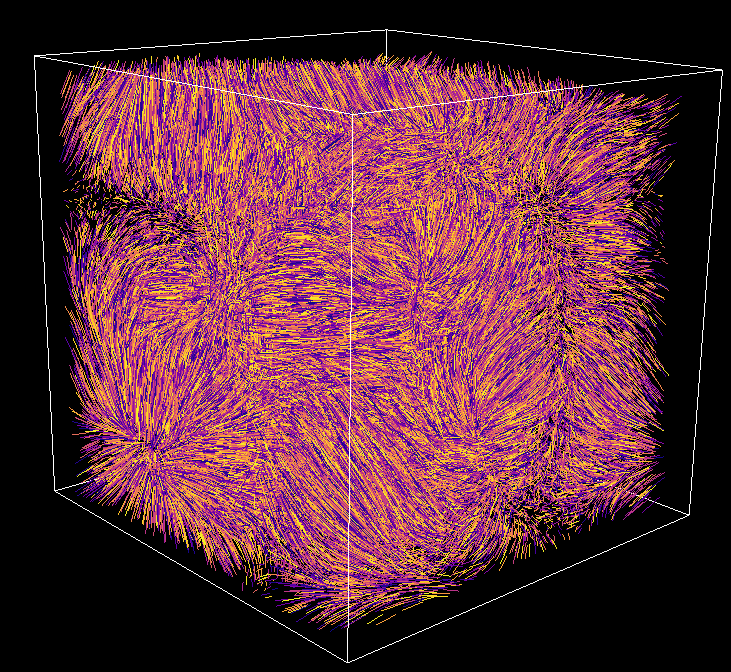
\includegraphics[height=4cm, keepaspectratio]{images/pathlines_nyx.png}
\caption{Nyx flow visualization}
\label{fig:pathlines_nyx}
\end{subfigure}
\hspace{-5mm}
\begin{subfigure}{0.32\textwidth}
\centering
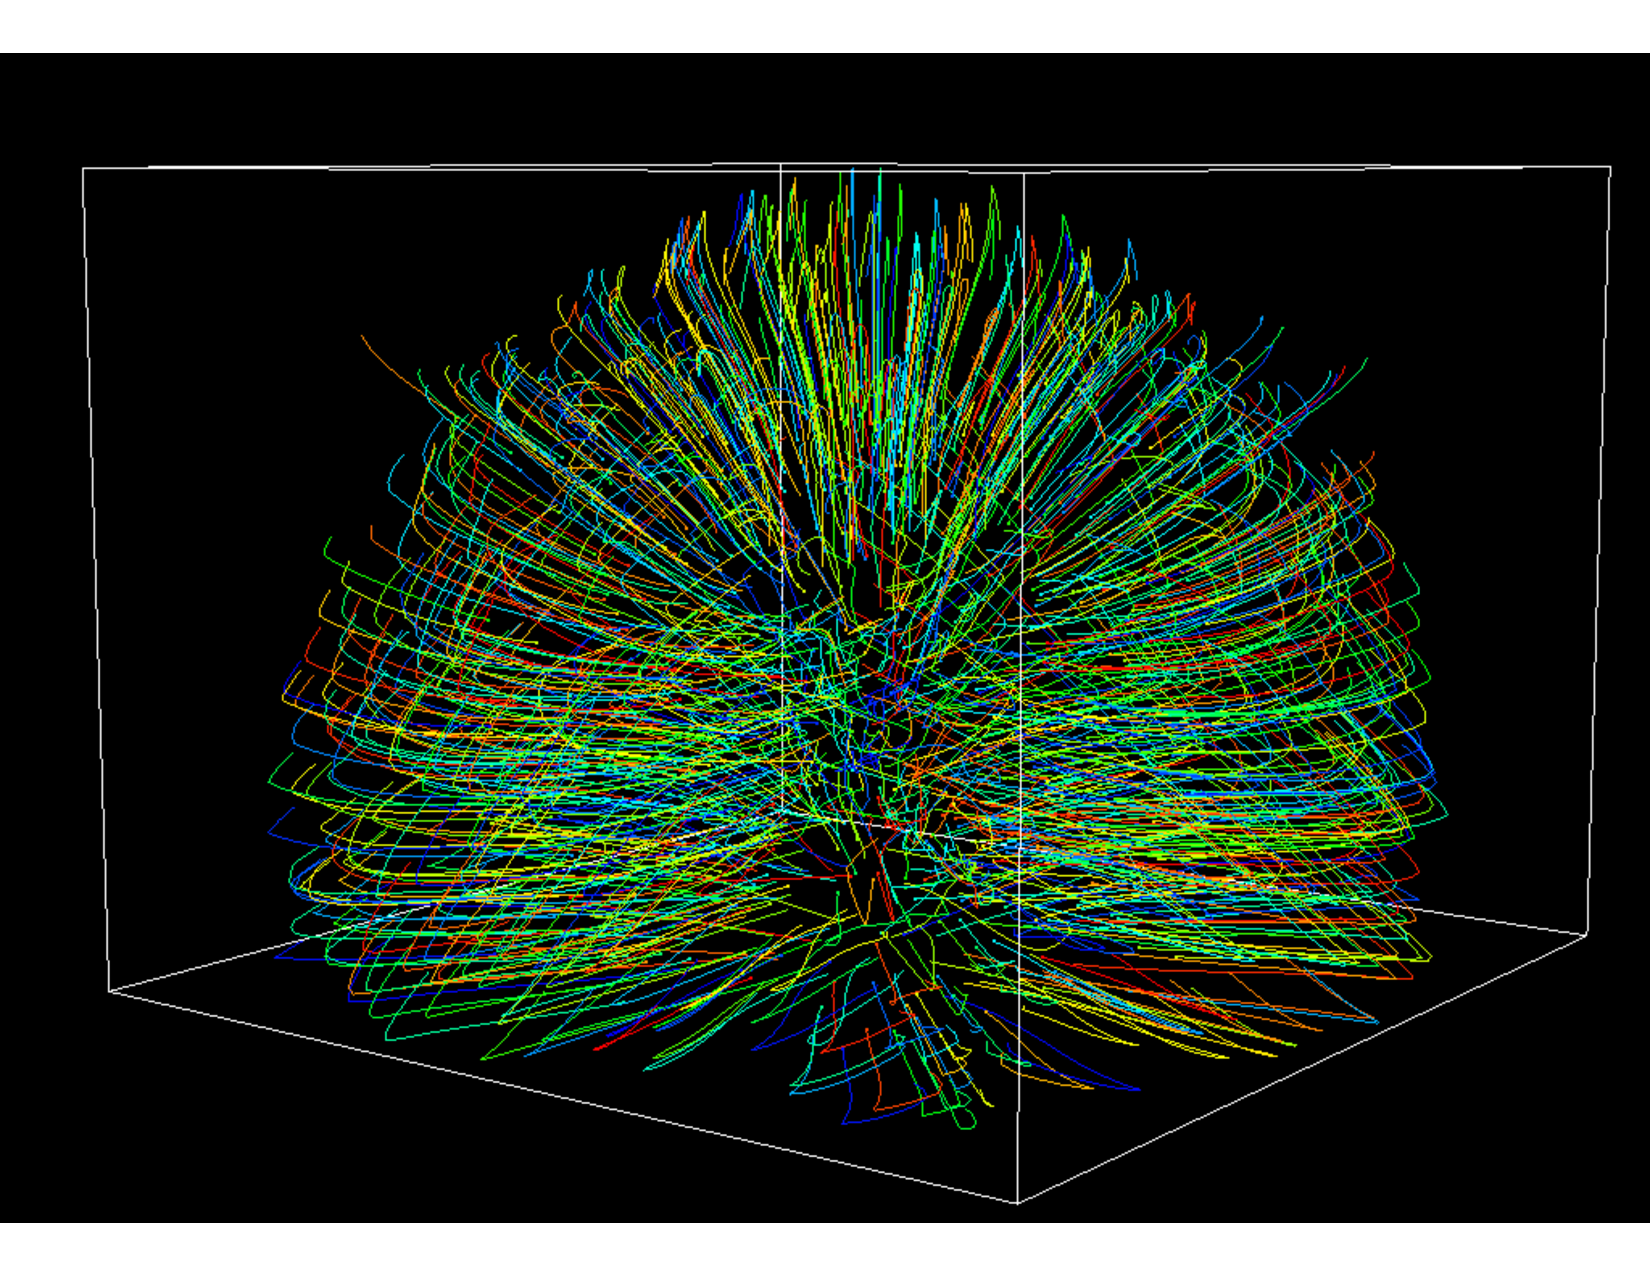
\includegraphics[height=4.36cm, keepaspectratio]{images/pathlines_clover.pdf}
\caption{Cloverleaf3D flow visualization}
\label{fig:pathlines_clover}
\end{subfigure}
\hspace{-5mm}
\begin{subfigure}{0.41\textwidth}
\centering
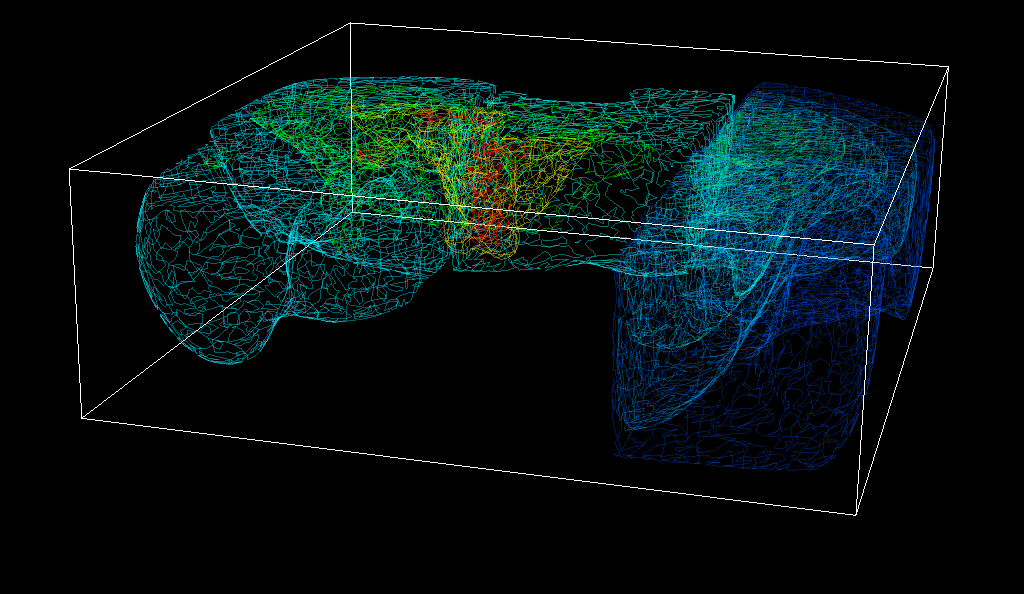
\includegraphics[height=4cm, keepaspectratio]{images/sw4_vis_2.png}
\caption{SW4 wave propagation visualization}
\label{fig:sw4_vis}
\end{subfigure}
\end{figure*}

\subsection{Datasets}
\label{sec:datasets}
For our study we consider three simulation application codes that are used and/or developed as part of the Exascale Computing Project efforts.
%

First, we use Cloverleaf3D which is a three-dimensional mini or proxy ECP application that solves compressible Euler equations in a hydrodynamics setting on a Cartesian grid using an explicit second-order method~\cite{cloverleaf3d}. 
%
Cloverleaf3D has been used developed and used by several studies to evaluate emerging architectures and various techniques targeting Exascale applications.
%
The simulation is initially relatively stable and begins with an energy bar expanding from the center of the XY plane along the Z-axis. 
%
Figure~\ref{fig:pathlines_clover} show pathlines calculated in the Cloverleaf3D domain that show this initial behavior in the simulation.

Next, we consider the SW4 seisomology simulation~\cite{petersson2015wave}.
%
This is an ECP application developed to study seismic wave propagation.
%
It operates and produces multiple domains with a time-dependent displacement field depending on the input deck provided to it.
%
We operate on a single domain and use the displacement vector field as input to our in situ Lagrangian operator.
%
Figure~\ref{fig:sw4_vis} is generated by visualizing the displacement magnitude of the particle trajectories extracted over the first X cycles of one of our simulation runs. 
%
The visualization uses line contours, with each node selecting 10 isovalues for the range of displacement magnitude in the node.
%
The color map range is the same for the entire domain, i.e., all nodes use the same maximum and minimum values.
%

The last data set we consider is the Nyx cosmology simulation~\cite{almgren2013nyx}, another ECP application.
%
The simulation's hydrodynamics is based on a compressible flow formulation in Eulerian coordinates. 
%
We built an Lya executable used to model Lyman-alpha forest in quasar spectra.
%
For this simulation, we derived the velocity field using the fields of momentum and density.
%
Figure~\ref{fig:vectorfield_nyx} shows a slice of the Nyx vector field at two time slices.
%
We observed that the unit vectors at each grid point remain relatively the same across all cycles.
%
The evolution of the vector field is in terms of velocity magnitude.
%
The maximum velocity magnitude in the domain increases steadily for every cycle of the application we simulated.
%
Further, Figure~\ref{fig:pathlines_nyx} is a visualization of the volume of the domain using 100,000 randomly seeded pathlines integrated for the first 25 cycles of the simulation.
%
\begin{figure}[h]
\centering
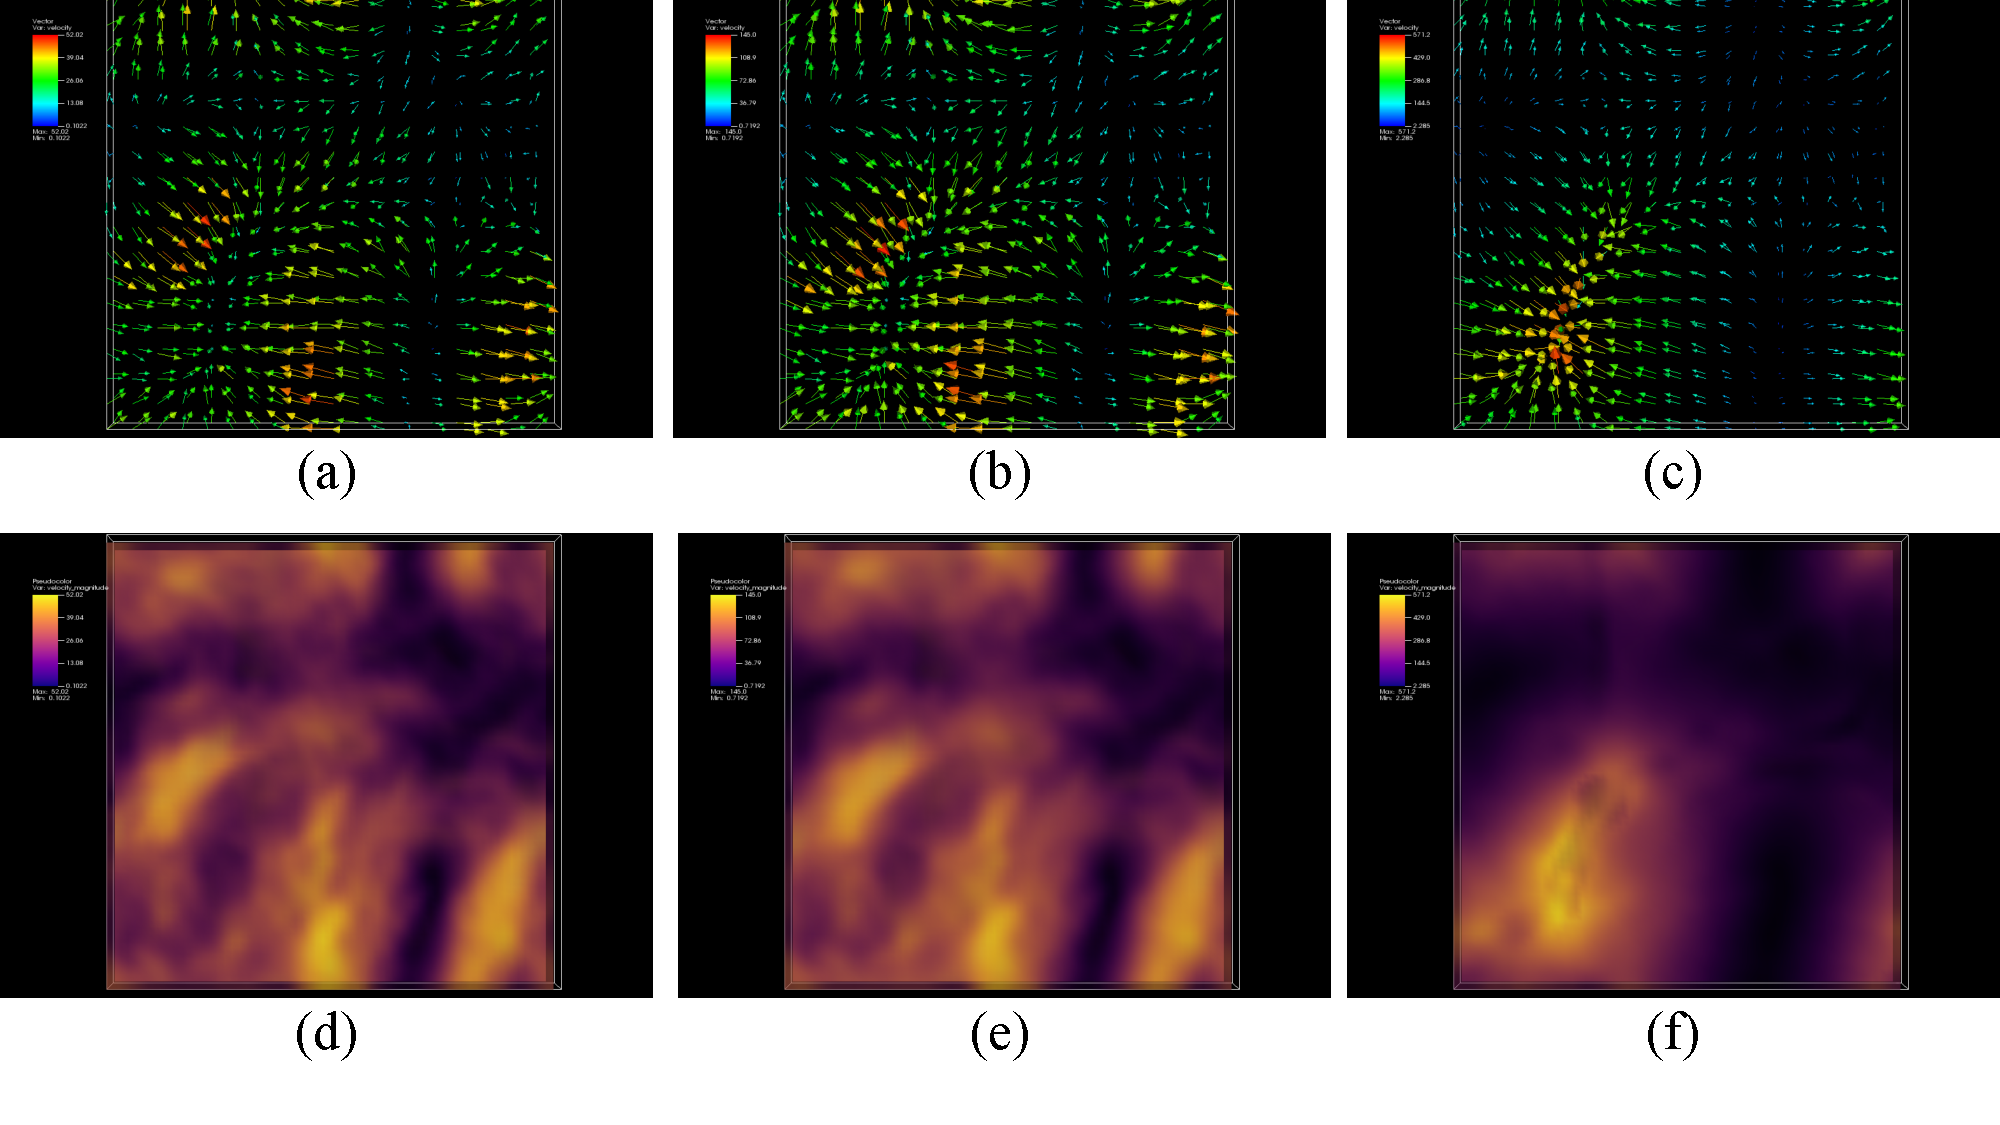
\includegraphics[width=1\linewidth, trim={0cm 1.1cm 0cm 0cm}, clip]{images/Nyx_vectorfields.pdf}
\vspace{-5mm}
\caption{Nyx vector field visualization: (a) and (d) show the vector field at time 0 and the maximum velocity magnitude is 52.02, (b) and (e) show the vector field at time 200 and the maximum velocity magnitude is 145.0, and finally, (c) and (f) show the vector field at time 400 and the maximum velocity is 571.2.}
\label{fig:vectorfield_nyx}
\vspace{-3mm}
\end{figure}





\subsection{In Situ Encumbrance}
\label{sec:encumbrance}

To evaluate the encumbrance placed on a simulation code, we measure and vary the various parameters that impact the cost associated with our implementation of in situ Lagrangian analysis.

\subsubsection{Computation and Memory Cost}

In situ Lagrangian analysis involves particle advection each cycle of the simulation. 
%
This introduces an overhead that depends on the complexity of the operation (we consider a simple approach; feature extraction or more complex seed placement would incur a cost), the implementation of particle advection, the number of particles being advected, and the underlying hardware.
%
Further, there are additional factors like number of MPI ranks on a node, the use of shared memory on a node, etc. 
%
For our study, we state when this is the case, i.e., multiple MPI ranks are operating on a single compute node.
%
We measure and report the average cost of particle advection per \textbf{Step} in terms of wall time and as a percentage of simulation time or DAV\%. 
%
This cost is averaged across all ranks and includes the costs of memory allocation and transfer.
%
Further, in situ Lagrangian analysis involves maintaining the state (current position) of particles in memory. 
%
We report the memory cost incurred on every MPI rank or compute node.

\subsubsection{I/O Cost}
In this empirical study, we do not report or factor the cost of I/O. 
%
We discuss our reasoning for this below. 

When writing to a binary format we observed very fast write times on Summit. 
%
Summit is designed to provide low access latency and high bandwidth. 
%
We found that a binary file of size 200 MB can be written in 0.0231 seconds on a single compute node running a single MPI task. 
%
And it takes 0.171 seconds of wall time for 6 MPI ranks to each write 200 MB files in parallel. 
%
In our experiments the largest file stored to disk by a single rank for a single interval or cycle is 115 MB. 
%
The range of sizes varies from 0.5 MB to 115 MB per node per instance of storing to disk (0.002 to 0.04 seconds, respectively). 
%
We provide some of these timings for reference in Table~\ref{table_binary}.
\begin{table}[h]
\centering
\vspace{-2mm}
\scalebox{0.9}{
\begin{tabular}{||c||c|c||}
\hline
File Size (MB) &  1 MPI/Node~(s) & 6 MPI/Node~(s) \\
\hline
1 & 0.0018 & 0.0022 \\
\hline
%5 & 0.0016 & 0.01 \\
%\hline
10 & 0.0032 & 0.0045 \\
\hline
%20 & 0.0054 & 0.0078 \\
%\hline
50 & 0.0064 & 0.013 \\
\hline
100 & 0.0125 & 0.038 \\
\hline
200 & 0.0231 & 0.171 \\
\hline
\end{tabular}
}
\vspace{-2mm}
\caption{Write time measurements for various file sizes (in binary format) to disk on Summit. We consider two cases: one MPI rank or six simultaneous MPI ranks each writing the file to disk on a single compute node. For each timing, we average over multiple runs and every timing is reported in seconds.}
\label{table_binary}
\vspace{-3mm}
\end{table}

%
Further, this infrequent operation and small cost of I/O in comparison 
to the cost of a particle advection step which is performed each cycle is small.

Although write times may be impacted at full scale --- all the nodes with several MPI ranks each trying to write at the same time - a study of this scale is beyond the scope of this work and more oriented toward a supercomputer I/O performance study. 
%
Further, in our relatively small study to inform ourselves, we found noise that we attribute to the cluster running hundreds of jobs simultaneously to be significant. 

Further, since \textbf{L-ISR} in intended to be used as a data reduction operator, the sizes of files written to disk would be approximately the same size (1:1) or significantly smaller (1:8, 1:27, 1:64). 
%
If I/O costs were to be impacted, either due to scale or file format type, then the cost of Eulerian would be more adversely affected if compared against a reduced Lagrangian I/O cost. 
%

Another point to consider is the infrastructure performing the operation of storing data. 
%
Depending on whether the data is being written to a burst buffer or some staging platform before moving data to permanent storage can significantly alter the value of these timings. 

All this being said, at scale scientists will not choose to save all the data due to excessive storage costs and since this would then indeed introduce a large cumulative encumbrance. 
%
Instead, they resort to temporal subsampling, i.e., saving data out at a predetermined frequency or at select cycles. 
%
One of our key assumptions is that as data sizes get larger, scientists will be forced to save less frequently or to store reduced data sets. 

\subsection{Accuracy Evaluation}
\label{sec:evaluation}
Our empirical study measures time-dependent vector field reconstruction error by evaluating the accuracy of test particles trajectories interpolated using the extracted Lagrangian representation.
%
For our Cloverleaf3D and Nyx experiments, we randomly place 100,000 and 50,000 test particles in the domain respectively.
%
For the SW4 experiments, we place 90,000 test particles in between $Z=5000$ and $Z=15,000$.
%

Our empirical study measures the L2-norm, i.e., the Euclidean distance, for each interpolated point and compares it to a ground truth that is precomputed using the complete simulation data. 
%
We use Avg$_{L2}$ to denote the average L2-norm and Max$_{L2}$ to denote the maximum L2-norm for an individual particle trajectory.
%
We note, that we observed in most cases, the Max$_{L2}$ was closely related to the end point distance between the ground truth and test particle trajectories.
%

An overall average of Avg$_{L2}$, denoted by AvgN$_{L2}$, is measured across $N$ test particle samples and provides a robust statistic~\cite{agranovsky2014improved, sane2018revisiting, sane2019interpolation, rapp2019void}.
%
Unlike AvgN$_{L2}$, a maximum error is more susceptible to outliers that could arise from small but complex regions of flow.
%
To provide a more detailed quantitative analysis compared to prior work, our empirical study uses histograms to capture the distribution of error~(Avg$_{L2}$, Max$_{L2}$) across all test particles and provides insight into per particle outcomes.  
